\newtheorem{definisi}{Definisi}

\chapter{Teori Permainan}
\section{Teori Permainan}
%bahas game theory
Teori permainan yang merupakan ilmu yang mempelajari pemodelan matematis untuk masalah dan kerja sama antara agen pengambil keputusan. Pengambil keputusan yang selanjutnya disebut sebagai pemain umumnya memiliki informasi yang berguna untuk proses pengambilan keputusan selanjutnya. Pemain harus mengetahui tiga hal yang mendasari masalah ini, seperti: Apa saja pilihan yang mungkin dilakukan? Apa saja hasil dari setiap pilihan? Bagaimana efek dari hasil tersebut (Tadelis, 2011)?

Pengamatan sederhana diatas memberikan definisi pertama yang penting untuk setiap masalah pengambilan keputusan.
\begin{definisi}
    \textbf{Masalah pengambilan keputusan} terdiri atas tiga komponen penting:
    \begin{enumerate}
        \item \textbf{Aksi}, yaitu seluruh alternatif pilihan yang dapat dilakukan pemain.
        \item \textbf{Payoff}, yaitu seluruh konsekuensi yang dapat terjadi dari aksi.
        \item \textbf{Preferensi}, yaitu deskripsi bagaimana pemain mengurutkan himpunan keluaran dari yang paling diinginkan hingga paling tidak diinginkan.
    \end{enumerate}
\end{definisi}

\begin{figure}
    \centering
    \tikzstyle{terminal} = [rectangle, rounded corners, draw=black, fill=blue!30, inner sep=.2cm, text width=3.5cm, align=flush center]
\tikzstyle{others} = [rectangle, text centered, draw=black, inner sep=.2cm, align=flush center, text width=2.5cm]
\tikzstyle{arrow} = [draw, thick, ->, >=stealth]

\newcommand{\factorcolor}{red!30}
\newcommand{\externalcolor}{cyan!10}
\newcommand{\payoffcolor}{green!20}

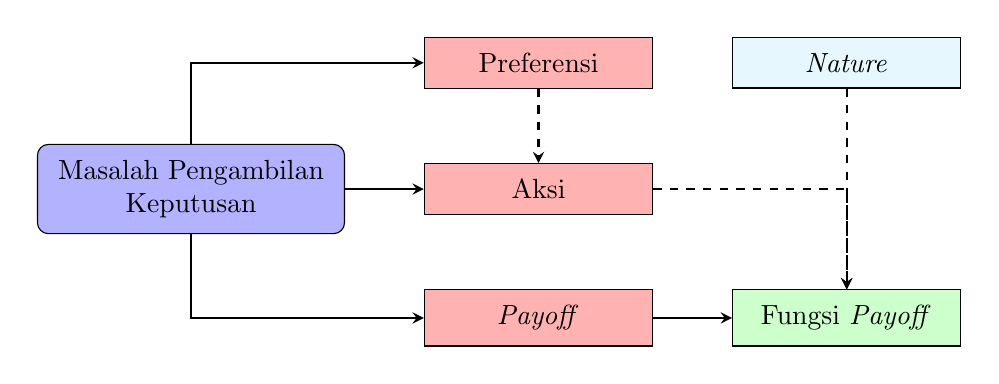
\begin{tikzpicture}[node distance=2cm]
  \matrix[column sep=1cm, row sep=7mm]{
                                                           & \node (pref) [others, fill=\factorcolor] {Preferensi};           &
    \node (nat) [others, fill=\externalcolor] {\textit{Nature}};                                                          \\
    \node (dp) [terminal] {Masalah Pengambilan Keputusan}; &
    \node (act) [others, fill=\factorcolor] {Aksi};        &                                                                    \\
                                                           & \node (po) [others, fill=\factorcolor] {\textit{Payoff}}; &
    \node (fpo) [others, fill=\payoffcolor] {Fungsi \textit{Payoff}};                                                    \\
  };

  \begin{scope}[every path/.style=arrow]
    \path (dp) -- (act);
    \path (dp) |- (pref);
    \path (dp) |- (po);
    \path (po) -- (fpo);
    \path [dashed] (pref) -- (act);
    \path [dashed] (act) -| (fpo);
    \path [dashed] (nat) -- (fpo);
  \end{scope}
\end{tikzpicture}
    \caption{Diagram Alir Masalah Pengambilan Keputusan}
\end{figure}
Relasi preferensi dinyatakan dalam notasi $\succsim$, yang menyatakan relasi antar \textit{payoff} yang dapat menunjukkan preferensi pemain. Sebagai contoh, misalkan terdapat seorang pemain yang ingin memilih rasa es krim vanila atau stroberi. Pilihan rasa es krim ini dapat di lambangkan sebagai himpunan aksi yang akan dipilih pemain yaitu  $A = \lbrace v, s\rbrace$, dimana $v$ menyatakan rasa vanila dan $s$ menyatakan rasa stroberi. Aksi yang dipilih pemain dapat berupa kondisi dimana pemain memutuskan untuk memakan es krim rasa vanila atau stroberi. Hal ini dapat ditulis sebagai himpunan bayaran $P = \lbrace V, S\rbrace$.
% Bab Studi Literatur digunakan untuk mendeskripsikan kajian literatur yang terkait dengan persoalan tugas akhir. Tujuan studi literatur adalah:

% \begin{enumerate}
%     \item menunjukkan kepada pembaca adanya gap seperti pada rumusan masalah yang memang belum terselesaikan,
%     \item memberikan pemahaman yang secukupnya kepada pembaca tentang teori atau pekerjaan terkait yang terkait langsung dengan penyelesaian persoalan, serta
%     \item menyampaikan informasi apa saja yang sudah ditulis/dilaporkan oleh pihak lain (peneliti/Tugas Akhir/Tesis) tentang hasil penelitian/pekerjaan mereka yang sama atau mirip kaitannya dengan persoalan tugas akhir.
% \end{enumerate}


% \section{Contoh Subbab}
% Perujukan literatur dapat dilakukan dengan menambahkan entri baru di berkas. Tulisan ini merujuk pada \parencite{knuth2001art,vasp1} atau \parencite{4026885} dan \parencite{Kim2006}

% Sekarang mau ke bab berapa yaaaa.... hmm... ke bab \ref{sec:latarbelakang} ahhhhh.

% \blindtext

% \subsection{Contoh Subsubbab}

% \blindtext

% \begin{figure}[h]
%     \centering
%     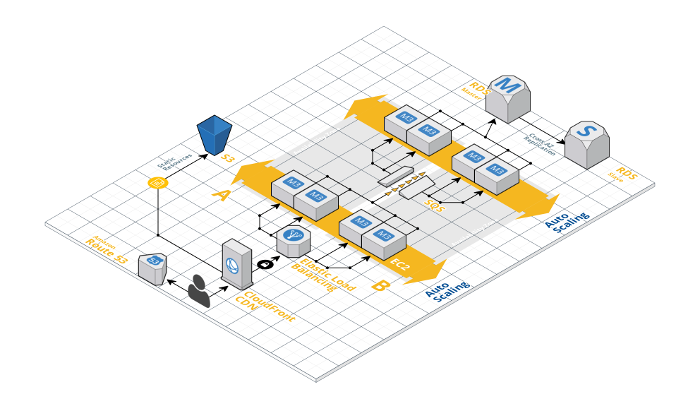
\includegraphics[width=0.8\textwidth]{chapter-2-infrastructure-diagram.png}
%     \caption{Contoh gambar}
% \end{figure}

% \subsubsection{Subsubsubbab}

% \blindtext

% \begin{table}[h]
%     \caption{Tabel random}
%     \vspace{0.25cm}
%     \begin{center}
%         \begin{tabular}{|c|c|c|c|}
%             \hline
%             Title1 & Title2 & Title3 & Title4  \tabularnewline
%             \hline
%             1647   & 1.97   & 0.68   & 1.90 \tabularnewline
%             2301   & 2.92   & 1.06   & 2.75 \tabularnewline
%             2969   & 3.23   & 1.16   & 3.78 \tabularnewline
%             3791   & 4.39   & 1.40   & 4.14 \tabularnewline
%             4625   & 6.72   & 1.87   & 5.59 \tabularnewline
%             \hline
%         \end{tabular}
%     \end{center}
% \end{table}

% \section{Menyisipkan Persamaan}

% Beberapa contoh menyisipkan persamaan.


% \subsection{Contoh Bikin Equation}
% \textbf{text tebal} dan ini \emph{miring}, bikin persamaan di baris yang sama, tinggal pake dolar2 $\Psi(\vec{r}_1,...,\vec{r}_N)$, sehingga persamaan Schr\"{o}dinger, terus, persamaan yang dinomeri kayak gini
% %ini contoh bikin persamaan, ..... :D
% \begin{equation}
%     \left[ \sum_{i}^{N}-\frac{\hbar^2}{2m}\nabla_i^2 + \sum_{i}^{N}V(\vec{r}_i)+ \sum_{i<j}^{N}(\vec{r}_i,\vec{r}_j)\right]\Psi = E\Psi
% \end{equation}

% untuk $N$-elektron, dengan $\hat{H}$=Hamiltonian, $E$=Energi total, $\hat{T}$=Energi kinetik, $\hat{V}$=Energi potensial, dan $\hat{U}$=Interaksi ektron-elektron.

% \subsection{Bikin Matrix}
% Lalalallala.... bikin matrix sekarang, yang ini dikecilin, pake smaller
%     {\smaller
%         \begin{equation}
%             \Psi({\bf r}_1, {\bf r}_2, \cdots {\bf r}_N) = \frac{1}{\sqrt{N!}}\left| \begin{array}{llcl}
%                 \phi_1({\bf r}_1)     & \phi_2({\bf r}_1)     & \cdots                & \phi_N({\bf r}_1)     \\
%                 \phi_1({\bf r}_2)     & \phi_2({\bf r}_2)     & \cdots                & \phi_N({\bf r}_2)     \\
%                 \phi_1({\bf r}_3)     & \phi_2({\bf r}_3)     & \cdots                & \phi_N({\bf r}_3)     \\
%                 \multicolumn{1}{c}{.} & \multicolumn{1}{c}{.} & \multicolumn{1}{c}{.} & \multicolumn{1}{c}{.} \\
%                 \multicolumn{1}{c}{.} & \multicolumn{1}{c}{.} & \multicolumn{1}{c}{.} & \multicolumn{1}{c}{.} \\
%                 \multicolumn{1}{c}{.} & \multicolumn{1}{c}{.} & \multicolumn{1}{c}{.} & \multicolumn{1}{c}{.} \\
%                 \phi_1({\bf r}_N)     & \phi_2({\bf r}_N)     & \cdots                & \phi_N({\bf r}_N)     \\
%             \end{array} \right|
%         \end{equation}
%     }

